\section{The engagement leak, measured}
\label{app:leak}

\begin{table}[H]
\centering\small
\begin{tabular}{@{}lccc@{}}
\toprule
split & impressions & matched to the later history block & history at or after the impression \\
\midrule
train & 168,522 & 144,087 & 143,998 (99.9\%) \\
val & 64,365 & 61,026 & 60,901 (99.8\%) \\
test & 244,647 & 244,647 & 0 (0.0\%) \\
\bottomrule
\end{tabular}
\caption{Future-click contamination in the engagement features before the fix
(Section~\ref{sec:q9}). Test was clean because it is drawn from the later block itself.}
\label{tab:leak}
\end{table}

\section{Full ablation grids}
\label{app:grids}

Each arm removes one feature and retrains the same model; \feat{stage1_only} keeps only the two
retrieval scores and \feat{pop_only} only click popularity. A positive ``full $-$ arm'' means the
removed feature helped. Bold marks intervals excluding zero. These grids were run before the
exposure features were added (17 features on \eb{}, 12 on \mind{}), which is why their full-model
AUC sits below the shipped system's.

\begin{table}[H]
\centering\scriptsize
\begin{tabular}{@{}lccc@{}}
\toprule
arm & val AUC & full $-$ arm, val [95\% CI] & full $-$ arm, test [95\% CI] \\
\midrule
full model & 0.7636 & & test AUC 0.7653 \\
stage1\_only & 0.5498 & \textbf{$+$0.2138} [$+$0.2110, $+$0.2168] & \textbf{$+$0.2223} [$+$0.2209, $+$0.2238] \\
pop\_only & 0.7348 & \textbf{$+$0.0288} [$+$0.0275, $+$0.0301] & \textbf{$+$0.0360} [$+$0.0352, $+$0.0367] \\
minus\_cat\_match & 0.7574 & \textbf{$+$0.0062} [$+$0.0053, $+$0.0071] & \textbf{$+$0.0069} [$+$0.0064, $+$0.0074] \\
minus\_n\_cands & 0.7580 & \textbf{$+$0.0056} [$+$0.0050, $+$0.0063] & \textbf{$+$0.0066} [$+$0.0062, $+$0.0069] \\
minus\_bm25 & 0.7625 & \textbf{$+$0.0011} [$+$0.0006, $+$0.0017] & \textbf{$+$0.0004} [$+$0.0001, $+$0.0007] \\
minus\_pop\_rank & 0.7629 & \textbf{$+$0.0007} [$+$0.0000, $+$0.0013] & \textbf{$+$0.0003} [$+$0.0000, $+$0.0006] \\
minus\_hist\_len & 0.7631 & \textbf{$+$0.0005} [$+$0.0000, $+$0.0010] & \textbf{$+$0.0005} [$+$0.0002, $+$0.0007] \\
minus\_pop\_velocity & 0.7632 & $+$0.0004 [$-$0.0001, $+$0.0008] & $-$0.0002 [$-$0.0004, $+$0.0001] \\
minus\_user\_scroll & 0.7632 & $+$0.0003 [$-$0.0001, $+$0.0008] & \textbf{$-$0.0003} [$-$0.0006, $-$0.0001] \\
minus\_age\_hours & 0.7632 & $+$0.0003 [$-$0.0001, $+$0.0008] & \textbf{$+$0.0004} [$+$0.0002, $+$0.0006] \\
minus\_engage\_sim & 0.7633 & $+$0.0003 [$-$0.0003, $+$0.0010] & \textbf{$+$0.0005} [$+$0.0002, $+$0.0008] \\
minus\_emb & 0.7637 & $-$0.0001 [$-$0.0006, $+$0.0004] & \textbf{$-$0.0003} [$-$0.0006, $-$0.0001] \\
minus\_emb\_rank & 0.7637 & $-$0.0001 [$-$0.0006, $+$0.0003] & $-$0.0001 [$-$0.0003, $+$0.0002] \\
minus\_pop\_24h & 0.7638 & $-$0.0003 [$-$0.0008, $+$0.0003] & $-$0.0001 [$-$0.0004, $+$0.0002] \\
minus\_ent\_overlap & 0.7639 & $-$0.0003 [$-$0.0008, $+$0.0002] & \textbf{$-$0.0006} [$-$0.0009, $-$0.0004] \\
minus\_pop\_rel\_max & 0.7639 & $-$0.0003 [$-$0.0009, $+$0.0003] & $+$0.0002 [$-$0.0002, $+$0.0005] \\
minus\_recency & 0.7639 & $-$0.0004 [$-$0.0008, $+$0.0001] & \textbf{$-$0.0005} [$-$0.0008, $-$0.0003] \\
minus\_user\_read & 0.7641 & \textbf{$-$0.0005} [$-$0.0010, $-$0.0000] & \textbf{$-$0.0006} [$-$0.0008, $-$0.0003] \\
minus\_pop\_causal & 0.7644 & \textbf{$-$0.0008} [$-$0.0013, $-$0.0003] & \textbf{$-$0.0006} [$-$0.0009, $-$0.0003] \\
\bottomrule
\end{tabular}

\caption{\eb{} small, 17-feature model, 64,365 val and 244,647 test impressions.}
\end{table}

\begin{table}[H]
\centering\scriptsize
\begin{tabular}{@{}lccc@{}}
\toprule
arm & val AUC & full $-$ arm, val [95\% CI] & full $-$ arm, test [95\% CI] \\
\midrule
full model & 0.6539 & & test AUC 0.6666 \\
pop\_only & 0.5475 & \textbf{$+$0.1064} [$+$0.1040, $+$0.1089] & \textbf{$+$0.0957} [$+$0.0935, $+$0.0978] \\
stage1\_only & 0.6372 & \textbf{$+$0.0167} [$+$0.0147, $+$0.0187] & \textbf{$+$0.0293} [$+$0.0274, $+$0.0313] \\
minus\_emb & 0.6497 & \textbf{$+$0.0042} [$+$0.0033, $+$0.0052] & \textbf{$+$0.0010} [$+$0.0001, $+$0.0018] \\
minus\_cat\_match & 0.6502 & \textbf{$+$0.0037} [$+$0.0028, $+$0.0047] & \textbf{$+$0.0070} [$+$0.0062, $+$0.0079] \\
minus\_bm25 & 0.6517 & \textbf{$+$0.0022} [$+$0.0013, $+$0.0031] & \textbf{$+$0.0027} [$+$0.0020, $+$0.0035] \\
minus\_hist\_len & 0.6530 & \textbf{$+$0.0008} [$+$0.0002, $+$0.0016] & $-$0.0001 [$-$0.0007, $+$0.0006] \\
minus\_pop\_causal & 0.6531 & \textbf{$+$0.0008} [$+$0.0001, $+$0.0014] & \textbf{$-$0.0009} [$-$0.0016, $-$0.0003] \\
minus\_pop\_velocity & 0.6534 & $+$0.0005 [$-$0.0003, $+$0.0013] & $+$0.0000 [$-$0.0007, $+$0.0007] \\
minus\_n\_cands & 0.6537 & $+$0.0001 [$-$0.0007, $+$0.0011] & \textbf{$+$0.0009} [$+$0.0002, $+$0.0017] \\
minus\_ent\_overlap & 0.6538 & $+$0.0001 [$-$0.0006, $+$0.0007] & $-$0.0005 [$-$0.0012, $+$0.0001] \\
minus\_pop\_rank & 0.6540 & $-$0.0001 [$-$0.0008, $+$0.0006] & $+$0.0003 [$-$0.0004, $+$0.0010] \\
minus\_pop\_rel\_max & 0.6541 & $-$0.0002 [$-$0.0010, $+$0.0007] & $+$0.0001 [$-$0.0007, $+$0.0009] \\
minus\_pop\_24h & 0.6542 & $-$0.0003 [$-$0.0010, $+$0.0004] & $+$0.0003 [$-$0.0003, $+$0.0010] \\
minus\_emb\_rank & 0.6542 & $-$0.0003 [$-$0.0010, $+$0.0004] & \textbf{$-$0.0007} [$-$0.0014, $-$0.0001] \\
\bottomrule
\end{tabular}

\caption{\mind{} small, 12-feature model, 61,894 val and 73,152 test impressions.}
\end{table}

\section{Beyond-accuracy metrics}
\label{app:beyond}

\begin{table}[H]
\centering\footnotesize
\begin{center}\pend{pending}: \texttt{q5\_beyond\_test} not generated yet\end{center}

\caption{Top-10 beyond-accuracy metrics, test split. Diversity is the share of top-10 pairs from
different categories; novelty is mean self-information in bits, so higher is less obvious;
coverage is the share of the catalogue that ever reaches a top 10. Coverage carries no interval
for the reason given in Section~\ref{sec:extended}.}
\end{table}

\section{Scaling measurements}
\label{app:scaling}

\begin{table}[H]
\centering\small
\begin{tabular}{@{}rrrrrrrr@{}}
\toprule
corpus & articles & FAISS MiB & BM25 p50 & exact kNN p50 & rerank p50 & total p50 & total p99 \\
\midrule
10\% & 2,074 & 6.1 & 0.24 & 0.79 & 2.33 & 3.94 & 7.28 \\
25\% & 5,184 & 15.2 & 0.40 & 1.66 & 2.20 & 4.99 & 8.42 \\
50\% & 10,369 & 30.4 & 0.69 & 3.13 & 2.35 & 7.00 & 10.22 \\
100\% & 20,738 & 60.8 & 3.93 & 21.11 & 17.66 & 46.87 & 109.00 \\
\bottomrule
\end{tabular}

\caption{Latency against corpus size in milliseconds, the numbers behind
Figure~\ref{fig:scaling}. Same machine and same model throughout.}
\end{table}

\section{Isolated-feature sweeps}
\label{app:sweeps}

Per-impression AUC of one feature used alone as the score, on val. An isolated score cannot be
absorbed by a correlated neighbour, which makes it a clean screen, but a winner here is only a
candidate: the popularity window gained $+$0.0447 in isolation and $+$0.0034 val inside the ranker.

\begin{table}[H]
\centering\small
\begin{tabular}[t]{@{}lcc@{}}
\toprule
popularity window & \eb{} & \mind{} \\
\midrule
1 h & 0.7082 & 0.5622 \\
6 h & 0.7349 & 0.5475 \\
24 h & 0.7254 & 0.5516 \\
72 h & 0.7045 & 0.5506 \\
168 h & 0.6902 & 0.5502 \\
unbounded & 0.6902 & 0.5502 \\
\bottomrule
\end{tabular}\hfill
\begin{tabular}[t]{@{}lcc@{}}
\toprule
min.\ scroll depth & AUC & history kept \\
\midrule
0\% & 0.5545 & 100.0\% \\
10\% & 0.5521 & 88.5\% \\
25\% & 0.5559 & 78.5\% \\
50\% & 0.5590 & 58.4\% \\
75\% & 0.5606 & 46.7\% \\
90\% & 0.5609 & 41.1\% \\
\bottomrule
\end{tabular}

\medskip
\begin{tabular}{@{}lcccccccc@{}}
\toprule
recency half-life & 1\,h & 3\,h & 6\,h & 12\,h & 24\,h & 48\,h & 96\,h & 168\,h \\
\midrule
\eb{} AUC & 0.5088 & 0.5087 & 0.5087 & 0.5088 & 0.5087 & 0.5088 & 0.5088 & 0.5088 \\
\bottomrule
\end{tabular}


\medskip
\begin{tabular}{@{}lcccccc@{}}
\toprule
history clicks & 1 & 5 & 10 & 20 & 50 & 100 \\
\midrule
uniform user vector & 0.5221 & 0.5368 & 0.5416 & 0.5483 & 0.5528 & 0.5545 \\
read-time weighted & 0.5221 & 0.5362 & 0.5434 & 0.5495 & 0.5554 & 0.5570 \\
\bottomrule
\end{tabular}

\caption{Top left: the click-popularity window. Top right: dropping history clicks with low scroll
depth (\eb{}, 100 clicks). Middle: the recency half-life, flat to four decimals over a 168$\times$
range. Bottom: history length and read-time weighting of the user vector on clean history.}
\end{table}

\section{Validation-split evaluation}
\label{app:val}

\begin{table}[H]
\centering\scriptsize
\begin{tabular}{@{}lccccc@{}}
\toprule
system & AUC & MRR & MRR, all clicks & nDCG@5 & nDCG@10 \\
\midrule
\multicolumn{6}{@{}l}{\textit{\eb{} small, val}} \\
BM25 (stage one) & \cellci{0.5205}{0.5180}{0.5231} & \cellci{0.3418}{0.3395}{0.3440} & \cellci{0.3414}{0.3391}{0.3436} & \cellci{0.3794}{0.3767}{0.3821} & \cellci{0.4607}{0.4586}{0.4629} \\[2pt]
embeddings (stage one) & \cellci{0.5506}{0.5482}{0.5530} & \cellci{0.3594}{0.3572}{0.3617} & \cellci{0.3589}{0.3567}{0.3612} & \cellci{0.4017}{0.3991}{0.4044} & \cellci{0.4778}{0.4757}{0.4801} \\[2pt]
fused (stage one) & \cellci{0.5528}{0.5503}{0.5553} & \cellci{0.3628}{0.3604}{0.3652} & \cellci{0.3623}{0.3600}{0.3647} & \cellci{0.4043}{0.4016}{0.4071} & \cellci{0.4807}{0.4785}{0.4830} \\[2pt]
two-stage re-ranker & \cellcib{0.7885}{0.7867}{0.7906} & \cellcib{0.5729}{0.5703}{0.5755} & \cellcib{0.5724}{0.5698}{0.5750} & \cellcib{0.6411}{0.6387}{0.6437} & \cellcib{0.6715}{0.6695}{0.6736} \\[2pt]
fused + lifetime popularity$^\ast$ & \cellci{0.5784}{0.5760}{0.5808} & \cellci{0.3707}{0.3684}{0.3731} & \cellci{0.3703}{0.3679}{0.3726} & \cellci{0.4184}{0.4159}{0.4210} & \cellci{0.4910}{0.4889}{0.4932} \\[2pt]
\midrule
\multicolumn{6}{@{}l}{\textit{\mind{} small, val}} \\
BM25 (stage one) & \cellci{0.5840}{0.5816}{0.5864} & \cellci{0.3204}{0.3176}{0.3232} & \cellci{0.2777}{0.2753}{0.2803} & \cellci{0.2924}{0.2895}{0.2954} & \cellci{0.3494}{0.3467}{0.3522} \\[2pt]
embeddings (stage one) & \cellci{0.6356}{0.6334}{0.6379} & \cellci{0.3422}{0.3396}{0.3449} & \cellci{0.2988}{0.2964}{0.3012} & \cellci{0.3202}{0.3175}{0.3231} & \cellci{0.3789}{0.3763}{0.3816} \\[2pt]
fused (stage one) & \cellci{0.6390}{0.6368}{0.6412} & \cellci{0.3478}{0.3450}{0.3504} & \cellci{0.3031}{0.3007}{0.3056} & \cellci{0.3248}{0.3220}{0.3275} & \cellci{0.3836}{0.3811}{0.3863} \\[2pt]
two-stage re-ranker & \cellcib{0.6997}{0.6976}{0.7018} & \cellcib{0.3977}{0.3950}{0.4005} & \cellcib{0.3422}{0.3397}{0.3448} & \cellcib{0.3729}{0.3701}{0.3759} & \cellcib{0.4313}{0.4287}{0.4339} \\[2pt]
\bottomrule
\end{tabular}

\caption{All accuracy metrics on val with 95\% intervals.}
\end{table}

\section{Reproducing the numbers}
\label{app:repro}

Every table in this note is generated from the results files by
\texttt{docs/design-note/make\_tables.py}; every measured number also has a row in
\texttt{docs/FACTS.md} or \texttt{docs/ABLATIONS.md} with the command that produced it.

\begin{small}
\begin{verbatim}
make venv && make download
python -m src.pipeline.split ebnerd_small        # one dataset per process
python -m src.retrieval.bm25 ebnerd_small
python -m src.retrieval.embeddings ebnerd_small
python -m src.retrieval.fuse ebnerd_small
python -m src.features.build ebnerd_small
python -m src.rerank.train ebnerd_small --tag final
python -m src.eval.run ebnerd_small --rerank-tag final
python -m src.eval.compare_reranks ebnerd_small ladder17 final
python -m src.eval.bench ebnerd_small --requests 2000 \
       --scale-points 0.1 0.25 0.5 1.0 --model-tag final
python -m src.eval.pool_size ebnerd_small
python -m pytest tests/
python -m src.submission.validate ebnerd submissions/ebnerd_predictions.zip
\end{verbatim}
\end{small}

\section{Leaderboard screenshots}
\label{app:screenshots}

\mind{}, Codabench competition 13967, submission 932812, user \texttt{namsyn}, rank 54,
scored 2026-09-19 09:23.

\begin{center}
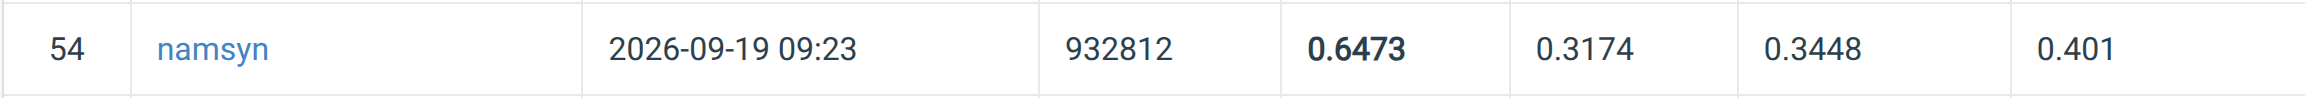
\includegraphics[width=\linewidth]{figures/mind-leaderboard-2026-09-19.png}
\end{center}

\eb{}, Codabench competition 2469: \textbf{no screenshot, and not for want of submitting.} The
prediction file was built, validated against all five structural checks, scored on a cluster node
in 3\,h\,06\,m and uploaded. It has not run. Codabench executes that competition on volunteered
compute workers, none were available, and the queue is first-come-first-served, so making a
machine available would not guarantee our own submission is the one it picks up. Producing this
screenshot is not within our control.

Nothing in this report depends on it: every \eb{} number quoted here is measured on our own
labelled test split, never on the leaderboard. The single thing we cannot state is an \eb{}
leaderboard rank, and we do not state one.
